\documentclass{article}
\usepackage{graphicx} % Required for inserting images
\usepackage{amsfonts}
\usepackage{tikz}
\usetikzlibrary{angles,quotes}
\usepackage{hyperref}
\usepackage{amsmath}
\usepackage{pgfplots}

\title{Complex and Quaternions}
\author{Intro to robotics}
\date{}

\begin{document}

\maketitle

\section{Introduction}
Why quaternions?\\
1. Solves gimbal lock.\\
2. More efficient calculations.\\
3. Unambiguous representation for orientations.

\section{2D complex rotations}
A complex number is of the form $a+bi$, where $a,b \in \mathbb{R}$  and $i \in \mathbb{C}$ and is often parameterized as an ordered (a,b), where b is the coefficient for complex number i.The vector 3+2i below represents a number in the complex plane. \\\\
\textbf{Definition: } $(-i)^2=i^2=-1 \text{ aka } \sqrt{-1}=i$\\\\
\begin{tikzpicture}
    \begin{scope}[thick,font=\scriptsize]   
    
    \draw [->] (-4,0) -- (4,0) node [above left]  {$\Re\{z\}$};
    \draw [->] (0,-4) -- (0,4) node [below right] {$\Im\{z\}$};
    
    \foreach \n in {-3,...,-1,1,2,...,3}{%
        \draw (\n,-3pt) -- (\n,3pt)   node [above] {$\n$};
        \draw (-3pt,\n) -- (3pt,\n)   node [right] {$\n i$};}
        
    \draw [->, thick, color=red] (0,0) -- (3,2);
    %\draw [color=blue, fill=blue] (2,3) circle(0.05);
    \node [color=red] at (3,2.5) {$c=3+2i=(3,2i)$};
\end{scope}
\end{tikzpicture}\newpage
Observe that whenever we multiply a vector by $i$ in the complex plane, that vector gets multiplied by 90 degrees. \\
\textbf{Example: }\\
start with complex number 3+2i, which is represented by the point (3,2i) in the complex plane, if we multiply it by $i$ we get:\\
$i(3+2i)=3i-2=-2+3i=(-2,3i)$ we can then keep multiplying the results by i, to continuously rotate by 90:\\
$i(-2+3i)=-2i-3=-3-2i=(-3,-2i)$\\
$i(-3-2i)=-3i+2=2-3i=(2,-3i)$\\
$i(2-3i)=2i+3=3+2i$ We are back where we started !!\\\\
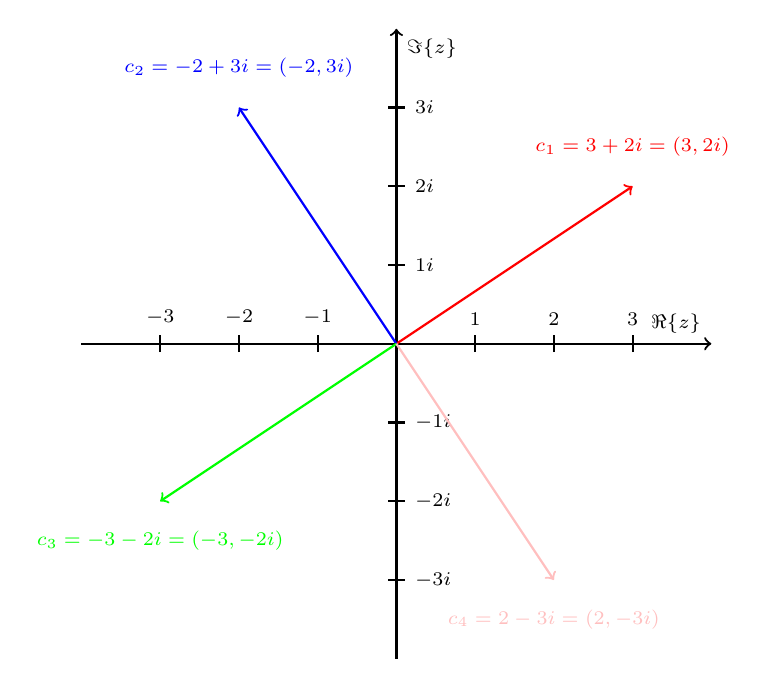
\begin{tikzpicture}
    \begin{scope}[thick,font=\scriptsize]   
    
    \draw [->] (-4,0) -- (4,0) node [above left]  {$\Re\{z\}$};
    \draw [->] (0,-4) -- (0,4) node [below right] {$\Im\{z\}$};
    
    \foreach \n in {-3,...,-1,1,2,...,3}{%
        \draw (\n,-3pt) -- (\n,3pt)   node [above] {$\n$};
        \draw (-3pt,\n) -- (3pt,\n)   node [right] {$\n i$};}
        
    \draw [->, thick, color=red] (0,0) -- (3,2);
    \draw [->, thick, color=blue] (0,0) -- (-2,3);
    \draw [->, thick, color=green] (0,0) -- (-3,-2);
    \draw [->, thick, color=pink] (0,0) -- (2,-3);
    \node [color=red] at (3,2.5) {$c_1=3+2i=(3,2i)$};
    \node [color=blue] at (-2,3.5) {$c_2=-2+3i=(-2,3i)$};
    \node [color=green] at (-3,-2.5) {$c_3=-3-2i=(-3,-2i)$};
    \node [color=pink] at (2,-3.5) {$c_4=2-3i=(2,-3i)$};
\end{scope}
\end{tikzpicture}

\section{Rotating by arbitrary angles using complex numbers}
Lets take an arbitrary point in the complex plane $c=(a+bi)$, and multiply it by the complex number $cos(\theta) + sin(\theta)i$, this will give us our vector c rotated by $\theta$.  \\\\
let $c = a+bi$ then $c_r= c * (cos(\theta) + sin(\theta)i) = (a+bi)(cos(\theta) + sin(\theta)i)$\\\\
Now let us foil this expression for the variable vector c to derive expressions we can use to avoid repeated multiplication.\\\\
$(cos(\theta)+sin(\theta)i)(a+bi)=acos(\theta)+bcos(\theta)i+asin(\theta)i-bsin(\theta)=acos(\theta)-bsin(\theta)+asin(\theta)i+bcos(\theta)i= \mathbf{(acos(\theta)-bsin(\theta), acos(\theta)i+bsin(\theta)i)}$\\\\
Notice that this gives us the same ordered set as matrix multiplication. Observe:\\
$v_r=R(\theta)v=\begin{bmatrix}
c\theta & -s\theta \\
s\theta & c\theta 
\end{bmatrix}\begin{bmatrix}
a\\
b
\end{bmatrix}=\begin{bmatrix}
ac\theta - bs\theta\\
as\theta + bc\theta
\end{bmatrix}$\\\\
\textbf{Example: } Rotate vector $c_1=(2,-2i)$ by $30^\circ$\\\\
$c_{1r}= (2*cos(30^{\circ})-(-2*sin(30^\circ)), 2*sin(30^\circ)i+-2*cos(30^\circ)i)=(2*.87-(-2*.5), 2*.5i + -2*.87i)=(2.74,-.74i)$\\\\
\begin{tikzpicture}
    \begin{scope}[thick,font=\scriptsize]   
    
    \draw [->] (-4,0) -- (4,0) node [above left]  {$\Re\{z\}$};
    \draw [->] (0,-4) -- (0,4) node [below right] {$\Im\{z\}$};
    
    \foreach \n in {-3,...,-1,1,2,...,3}{%
        \draw (\n,-3pt) -- (\n,3pt)   node [above] {$\n$};
        \draw (-3pt,\n) -- (3pt,\n)   node [right] {$\n i$};}
        
    \draw [->, thick, color=black] (0,0) -- (2,-2);
    \draw [->, thick, color=red] (0,0) -- (2.74,-.74);
    \node [color=black] at (2,-2.5) {$c_1=2-2i=(2,-2i)$};
    \node [color=red] at (2.74,-1.25) {$c_{1r}=-2+3i=(2.74,-.74i)$};
\end{scope}
\end{tikzpicture}

\section{e}
Eulers number, $e$ was discovered by Euler; the same guy from Eulers angle. It is roughly equal to $e=2.718 ...$ and it has a few cool properties.\\\\
\textbf{1. } The natural logs base is eulers number. \\
\textbf{2. }$e = lim_{x \xrightarrow{} \infty} (1 + \frac{1}{x})^x$\\
\textbf{3. } $e^{\theta i}$ can be approximated by taylor series to be $exp(\theta i )= 1+\frac{\theta i}{1!}+\frac{(\theta i)^2}{2!}
\frac{(\theta i)^3}{3!}+\frac{(\theta i)^4}{4!}+...$\\
\textbf{4. } $e^{\theta i}=cos(\theta)+sin(\theta)i$, this can be related to \textbf{3.} because the taylor series for $cos(\theta)$ plus the taylor series of $sin(\theta)i$ is equivalent to the taylor series for $e^{\theta i}$, you can google for proof.\\
\textbf{5. } This means $e^{\theta i}v=v_r$, vector v is rotated by $\theta$ and turns into $v_r$

\section{Matrices for complex numbers}
We can also represent complex multiplication with matrices, for example if I want to represent $(a+bi)(c+di)$ then it would be:\\
$\begin{bmatrix}
a & -b\\
b & a
\end{bmatrix}\begin{bmatrix}
c \\
d
\end{bmatrix}=\begin{bmatrix}
ac-bd \\
bc+ad
\end{bmatrix}$\\\\
Notice that this is the same formula used above for representing complex numbers with an ordered pair$(ac-bd,bci+adi)$!\\\\
We can also represent i as a matrix, let i = 0+1i, then using or formula above, a = 0 and b = 1; then:\\
$\begin{bmatrix}
a & -b\\
b & a
\end{bmatrix}=\begin{bmatrix}
0 & -1\\
1 & 0
\end{bmatrix}$\\\\
We can then prove that this works by showing $i^2=1$\\\\
$\begin{bmatrix}
0 & -1\\
1 & 0
\end{bmatrix}\begin{bmatrix}
0 & -1\\
1 & 0
\end{bmatrix}=-1\begin{bmatrix}
1 & 0\\
0 & 1
\end{bmatrix}$\\\\
\textbf{Rotation example}
rotate $c=-1.14+2.5i$ by $80^\circ$ using complex matrices.\\
$(cos(\theta) + sin(\theta)i)(a+bi)=\begin{bmatrix}
a & -b\\
b & a
\end{bmatrix}\begin{bmatrix}
a \\
b
\end{bmatrix}=\begin{bmatrix}
ac-bd \\
bc+ad
\end{bmatrix}=\begin{bmatrix}
c80^\circ & -s80^\circ\\
s80^\circ & c80^\circ
\end{bmatrix}\begin{bmatrix}
-1.14\\
2.5
\end{bmatrix}=\begin{bmatrix}
-2.64 \\
-.69
\end{bmatrix}$\\\\
\begin{tikzpicture}
    \begin{scope}[thick,font=\scriptsize]   
    
    \draw [->] (-4,0) -- (4,0) node [above left]  {$\Re\{z\}$};
    \draw [->] (0,-4) -- (0,4) node [below right] {$\Im\{z\}$};
    
    \foreach \n in {-3,...,-1,1,2,...,3}{%
        \draw (\n,-3pt) -- (\n,3pt)   node [above] {$\n$};
        \draw (-3pt,\n) -- (3pt,\n)   node [right] {$\n i$};}
        
    \draw [->, thick, color=black] (0,0) -- (-1.14,2.5);
    \draw [->, thick, color=red] (0,0) -- (-2.64,-.69);
    \node [color=black] at (-1.14,2.75) {$c=-1.14+2.5i=(-1.14,2.5i)$};
    \node [color=red] at (-2.64,-.9) {$c_{r}=-2.64+.69i=(-2.64,-.69i)$};
\end{scope}
\end{tikzpicture}
\section{Complex Conjugate}
The conjugate of a complex number is the complex number that satisfies the equation $c*c^*=real number(no complex component)$. This number is easy to compute. If $c=a+bi$ then $c^*=a-bi$, we can show:\\\\
$(a+bi)(a-bi)=a^2-abi+abi-b^2(-1)=a^2+b^2$\\
\textbf{Example: }\\
Given $35.3+2.718i$ the complex conjugate is $35.3-2.718i$; $(35.3+2.718i)(35.3-2.718i)=1246.09+95.95i-95.95i-7.39(-1)=1246.09+7.39=1253.48$

\section{Quaternions}
\label{sec:Q}
Quaternions are an extension on the complex numbers, just like the complex numbers introduced the number $i$; the quaternion numbers include the number $i$ and add two additional numbers $j$ and $k$ such that:\\\\
$i^2=j^2=k^2=ijk=-1$ and \\\\
\begin{tabular}{ |p{3cm}|p{3cm}|p{3cm}| p{3cm} |}
\hline
\multicolumn{4}{|c|}{Multiplication Rules for Quaternions} \\
\hline
 & \textbf{i} & \textbf{j} & \textbf{k} \\
\hline
\textbf{i} & -1 & k & -j\\
\textbf{j} & -k & -1 & i\\
\textbf{k} & j & -i & -1\\
\hline
\end{tabular}\\
\textbf{Numbers i,j and k do not follow the commutative property.}
\subsection{Quaternions representations}
Just like complex numbers we have three ways to represent quaternions. \\
\textbf{1. } Algebraically: $a + bi + cj + dk$,  where $a,b,c,$ and $d$ are real numbers.\\\\
\textbf{2. } As an ordered set: $(a,b,c,d)$, such that (scalar real component, scalar for i component,scalar for j component, scalar for k component)\\\\
\textbf{3. }Matrix representation: $\begin{bmatrix}
a & -b & -c & -d\\
b & a & -d & c\\
c & d & a & -b \\
d & -c & b & a
\end{bmatrix}$ (More on this later)

\subsection{Quaternion Multiplication}
Consider $q_1$ and $q_2$ such that $q_1$ and $q_2$ are quaternions. Then $q_1 * q_2 =$(simplify with multiplication rules from table):\\\\
$q_1 * q_2 = (a+bi+cj+dk)(e+fi+gj+hk)=ae+afi+agj+ahk+
                                      bei+bfi^2+bgij+bhik+
                                      cej+cfji+cgj^2+ckhj+
                                      dek+dfki+dgkj+dhk^2= ae+afi+agj+ahk+
                                                           bei-bf+bgk-bkj+
                                                           cej-cfk-cg+chi+
                                                           dek+dfj-dgi-dh$ (Algebraic form)\\\\
We can then reorganize the terms to represent this number as an ordered set. \\
$q_1*q_2=\\(ae-bf-cg-dh,\\ be+af-dg+ch,\\ ce+df+ag-bh,\\ de-cf+bg+ah)$\\\\
\textbf{Things to keep in mind}\\
1. Just like matrix multiplication, quaternion multiplication is not commutative, $q_1q_2 \neq q_2q_1$.\\
2. However , it is associative, $(q_1q_2)q_3=q_1(q_2q_3)$. \\\\
\textbf{Quaternion as scalar-vector ordered pair}\\
Let $q=(a+bi+cj+dk)$, we can reparameterize a quaternion as:\\ $q=(w=a, v=\begin{bmatrix}
b\\
c\\
d
\end{bmatrix})$\\\\
now we can express quaternion multiplication as:\\ $q_1q_2=(w_1w_2-v_1 \cdot v_2, w_1v_2+w_2v_1+v_1 \times v_2)$\\\\
\textbf{Example:}\\\\
Let $q_1=(a,b,c,d)=(1,2,3,4)$ and $q_2=(e,f,g,h)=(0,5,6,0)$ so,\\
$q_1q_2=\begin{pmatrix}
ae-bf-cg-dh,\\
be+af-dg+ch,\\
ce+df+ag-bh,\\ 
de-cf+bg+ah
\end{pmatrix}=\begin{pmatrix}
1*0-2*5-3*6-4*0,\\
2*0+1*5-4*6+3*0,\\
3*0+4*5+1*6-2*0,\\
4*0-3*5+2*6+1*0
\end{pmatrix}=\begin{pmatrix}
-28,-19,26,-3
\end{pmatrix}$\\\\
\textbf{Alternatively:}\\
$v_1 \times v_2 = \begin{bmatrix}
-24\\
20\\
-3
\end{bmatrix}$\\
$q_1 = (w_1=1, v_1=\begin{bmatrix}
2\\
3\\
4
\end{bmatrix})$  and $q_2 = (w_2=0, v_2=\begin{bmatrix}
5\\
6\\
0
\end{bmatrix})$ then ,\\ $q_1q_2=(w_1w_2 - v_1 \cdot v_2, w_1v_2 + w_2v_1 + v_1 \times v_2)=\\
(1*0-(2*5+3*6+4*0),1*\begin{bmatrix}
5\\
6\\
0
\end{bmatrix}+0*\begin{bmatrix}
2\\
3\\
4
\end{bmatrix}+\begin{bmatrix}
-24\\
20\\
-3
\end{bmatrix} )=(-28, \begin{bmatrix}
-19\\
26\\
-3
\end{bmatrix})$\newpage
\section{Matrix representation for quaternions}
Consider: $q_1q_2=\begin{pmatrix}
ae-bf-cg-dh,\\
be+af-dg+ch,\\
ce+df+ag-bh,\\ 
de-cf+bg+ah
\end{pmatrix}$ We can represent this ordered set multiplication as : \\
$\begin{bmatrix}
a & -b & -c & -d\\
b & a & -d & c\\
c & d & a & -b\\
d & -c & b & a
\end{bmatrix}\begin{bmatrix}
e\\
f\\
g\\
h
\end{bmatrix}$\\\\
\textbf{Example: } Let $q_1= (3,-7,2,-2)$ and $q_2=(-23, 0, 24, 8)$\\\\
$\begin{bmatrix}
a & -b & -c & -d\\
b & a & -d & c\\
c & d & a & -b\\
d & -c & b & a
\end{bmatrix}\begin{bmatrix}
e\\
f\\
g\\
h
\end{bmatrix}=
\begin{bmatrix}
3 & 7 & -2 & 2\\
-7 & 3 & 2 & 2\\
2 & -2 & 3 & 7\\
-2 & -2 & -7 & 3
\end{bmatrix}\begin{bmatrix}
-23\\
0\\
24\\
8
\end{bmatrix}=
\begin{bmatrix}
-101\\
225\\
82\\
-98
\end{bmatrix}$

\subsection{Identity matrices for quaternions}
$i = (0,1,0,0)=\begin{bmatrix}
0 & -1 & 0 & 0\\
1 & 0 & 0 & 0\\
0 & 0 & 0 & -1\\
0 & 0 & 1 & 0
\end{bmatrix}$\\\\
$j = (0,0,1,0)=\begin{bmatrix}
0 & 0 & -1 & 0\\
0 & 0 & 0 & 1\\
1 & 0 & 0 & 0\\
0 & -1 & 0 & 0
\end{bmatrix}$\\\\
$k = (0,0,0,1)=\begin{bmatrix}
0 & 0 & 0 & -1\\
0 & 0 & -1 & 0\\
0 & 1 & 0 & 0\\
1 & 0 & 0 & 0
\end{bmatrix}$\\\\
You can verify that for the matrices above that:\\
$i^2 = j^2= k^2 = ijk =-1$ and all the rules from the quaternion multiplication table from \hyperref[sec:Q]{section 7}.

\section{Quaternion Conjugates and Inverses}
The \textbf{conjugate} of a quaternion $q$ is the quaternion $q^*$ such that $qq^*=(s,0,0,0)$ where s is a scalar. In other words, a quaternion multiplied by its conjugate is just a real number(no i,j, or k component). Just like complex numbers we get the conjugate by negating all the non-real components of the quaternion. So given:\\\\
if $q=(a,b,c,d)$ then $q^*=(a,-b,-c,-d)$\\\\
The \textbf{inverse} of a quaternion $q$ is similar to its conjugate, and satisfies the equation $qq^{-1}=(1,0,0,0)$.\\\\
To compute the inverse of $q$ use the formula $\frac{q^*}{|q|}$\\\\
Something else to note if we imagine $q$ being a vector in quaternion space(cant visualize since it would be 4-dimensional space with orthogonal axes real, i,j, and k), then the magnitude $q$ is actually encoded in $qq^*=(s,0,0,0)$ where $\sqrt{s}$ is the magnitude of $q$.We can see this in:\\\\
$\begin{bmatrix}
a & -b & -c & -d\\
b & a & -d & c\\
c & d & a & -b\\
d & -c & b & a
\end{bmatrix}\begin{bmatrix}
a\\
-b\\
-c\\
-d
\end{bmatrix}=\begin{bmatrix}
a^2 + (-b)^2 + (-c)^2 + (-d)^2\\
ab + -ba + -c-d + -dc\\
ac + -bd + -ca + -d-b \\
ad + -b-c + -cb + -da 
\end{bmatrix}=\begin{bmatrix}
a^2 + b^2 + c^2 + d^2\\
0\\
0\\
0
\end{bmatrix}$ Notice that the terms in the i,j and k row all cancel out and equal 0. If you take the $\sqrt{a^2+b^2+c^2+d^2}$ you can see that its the same function as the magnitude of a vector! \\\\
\textbf{Example: }\\
Let $q=(-3.14,2.718, 1.618,-.618)$ then $q^*=(-3.14, -2.718,-1.618,.618)$ \\
$qq^*=(-3.14^2+2.718^2+1.618^2+-.618^2,0,0,0)=(9.86+7.39+2.62+.38,0,0,0)=(20.25,0,0,0)$\\\\
Then the inverse $q^{-1}=\frac{q^*}{\sqrt{20.25}}=(\frac{-3.14}{\sqrt{20.25}}, \frac{-2.718}{\sqrt{20.25}},\frac{-1.618}{\sqrt{20.25}},\frac{.618}{\sqrt{20.25}})$

\section{Converting Euler angles and rotation matrices to quaternions $(q_{rot})$}
Let $n$ be the axis of rotation: $n = \begin{bmatrix}
n_1\\
n_2\\
n_3
\end{bmatrix}$\\
Let quaternion $e^{\theta n }= cos(\theta)+sin(\theta)n_1i+sin(\theta)n_2j+sin(\theta)n_3k$(this is our rotational quaternion)\\
(If interested, reference taylor expansion approximation for eulers number to see how this formula is derived.)\\\\
For now let us consider the three rotational axes we are familiar with: \\\\
$n_x = \begin{bmatrix}
1\\
0\\
0
\end{bmatrix}\text{(Rotates on yz plane), }(R_x), 
n_y = \begin{bmatrix}
0\\
1\\
0
\end{bmatrix}\text{(Rotates on xz plane), }(R_y), \\
n_z = \begin{bmatrix}
0\\
0\\
1
\end{bmatrix}\text{(Rotates on xy plane)}(R_z)$\\\\
\textbf{The problem we are trying to solve is given $R_{z'y'x'}$ find the equivalent quaterion($q_{rot}$)}\\\\
In general $R_{z'y'x'}(\alpha,\beta,\gamma)=e^{\frac{\alpha}{2} n_z}e^{\frac{\beta}{2} n_y}e^{\frac{\gamma}{2} n_x}$\\\\
\textbf{Example: } Convert the rotation matrix $R_{z'y'x'}(68^\circ,122^\circ,248^\circ)$ to its equivalent quaternion.\\\\
$R_{z'y'x'}(68^\circ,122^\circ,248^\circ) \rightarrow e^{\frac{68}{2} n_z}e^{\frac{122}{2} n_y}e^{\frac{248}{2} n_x}=(cos(34)+ sin(34)k)(cos(61)+ sin(61)j)(cos(124)+ sin(124)i)=.15 +.6i -.2j -.76k$

\section{Rotating vectors using quaternions}
To rotate a vector $v$ by theta on some rotational axis, we use the formula :\\\\
$v_r  = q_{rot}vq_{rot}^*$\\\\
\textbf{Example \#1: } Rotate vector $v=\begin{bmatrix}
-2\\
7\\
2
\end{bmatrix}$ on the xz plane by $40^\circ$\\\\
$n = n_x = \begin{bmatrix}
0\\
1\\
0
\end{bmatrix}$ now we can use the formula:\\
First we compute $q_rot$ which is just $q_rot=e^{\frac{40^\circ}{2} n_x }=cos(20^\circ) + 0*sin(20^\circ)i + 1*sin(20^\circ)j + 0*sin(20^\circ)k=cos(20^\circ)+sin(20^\circ)j$\\\\
and  $q_{rot}^*=cos(20^\circ)-sin(20^\circ)j$\\\\
Now we use the rotation formula:\\
$q_{rot}vq_{rot}^*=(cos(20^\circ)+sin(20^\circ)j) (-2i+7j+2k) (cos(20^\circ)-sin(20^\circ)j)$\\
\textbf{Once simplified use any of the three quaternion multiplication techniques: foil, matrix, ordered pair, or scalar-vector ordered pair }\\\\
\textbf{Quaternion Matrix Multiplication}\\
We must do two matrix quaternion multiplication to get our answer, first we do $(cos(20^\circ)+sin(20^\circ)) (-2i+7j+2k)$:\\
$\begin{bmatrix}
c20 & 0 & -s20 & 0\\
0 & c20 & 0 & s20\\
s20 & 0 & c20 & 0\\
0 & -s20 & 0 & c20
\end{bmatrix}\begin{bmatrix}
0\\
-2\\
7\\
2
\end{bmatrix}=\begin{bmatrix}
-2.4\\
-1.2\\
6.58\\
2.56
\end{bmatrix}$\\\\
Now we have $(cos(20^\circ)+sin(20^\circ)j) (-2i+7j+2k) (cos(20^\circ)-sin(20^\circ)j)=(-2.4-1.2i+6.58j+2.56k)(cos(20^\circ)-sin(20^\circ)j)$ so we do one more matrix quaternion multiplication:\\
$\begin{bmatrix}
-2.4 & 1.2 & -6.58 & -2.56\\
-1.2 & -2.4 & -2.56 & 6.58\\
 6.58 & 2.56 & -2.4 & 1.2\\
 2.56 & -6.58 &  -1.2 & -2.4 
\end{bmatrix}\begin{bmatrix}
c20\\
0\\
-s20\\
0
\end{bmatrix}=\begin{bmatrix}
0\\
-.25\\
7\\
2.82
\end{bmatrix}$\\\\\\
\textbf{Example \#2: } Rotate vector $v=\begin{bmatrix}
2\\
-1\\
2
\end{bmatrix}$ by $100^\circ$ on xy plane then $35^\circ$ on xz plane.\\\\
First we compute $q_rot$ which is:\\\\ 
$q_{rot}=e^{35^\circ\begin{bmatrix}
0\\
1\\
0
\end{bmatrix}}*e^{100^\circ\begin{bmatrix}
0\\
0\\
1
\end{bmatrix}}=(cos(35^\circ)+sin(35^\circ)j)(cos(100^\circ)+sin(100^\circ)k)=0.613 +0.230i +0.193j +0.731k$\\
Now that we have computed $q_{rot}$ we can use use the rotation formula $q_{rot}vq_{rot}^*$ to get $v_r$:\\\\
$v_r=q_{rot}vq_{rot}^*=(0.613 +0.230i +0.193j +0.731k)(0+2i-1j+2k)(0.613 -0.230i -0.193j -0.731k)=0+1.67i+2.14j+1.27k$\\\\
We got this by using quaternion matrix multiplication:\\
$\begin{bmatrix}
.613 & -.230 & -.193 & -.731\\
.230 & .613 & -.731 & .193\\
 .193 & .731 & .613 & -.230\\
 .731 & -.193 &  .230 & .613 
\end{bmatrix}\begin{bmatrix}
0\\
2\\
-1\\
2
\end{bmatrix}=\begin{bmatrix}
-1.73\\
2.34\\
0.39\\
0.61
\end{bmatrix}$\\\\
$\begin{bmatrix}
-1.73 & -2.34 & -.39 & -.61\\
2.34 & -1.73 & -.61 & .39\\
 .39 & .61 &  -1.73 & -2.34\\
 .61 & -.39 &  2.34 & -1.73 
\end{bmatrix}\begin{bmatrix}
.613\\
-.230\\
-.193\\
-.73
\end{bmatrix}=\begin{bmatrix}
0\\
1.67\\
2.14\\
1.27
\end{bmatrix}$

\section{Quaternions to rotation matrices}
\begin{figure}[htp]
    \includegraphics[width=12cm]{quat_to_euler.png}
    \label{fig:mainy}
\end{figure} \\
\end{document}
